\documentclass[12pt]{amsart}
\usepackage[symbol]{footmisc}
\usepackage{float}

\usepackage{style_template}
\renewcommand*{\thefootnote}{\fnsymbol{footnote}}

% \newtheorem{theorem}{Theorem}
% \newtheorem{definition}{Definition}

\title{UMD Fairness Research Group Meeting Notes}
\author{David Yang}
\date{Summer 2023}

\begin{document}

\maketitle

\begin{center}
    Note: $\dagger$ denotes equal contribution.
\end{center}

\section{Bilevel Optimization Problems in ML and Efficient Solvers (June 15th)}

\textit{Led by Mucong Ding.} \\

\begin{definition}[Bilevel Optimization]
The \textbf{Bilevel Optimization} problem is 
\[\min_{v, \theta} f(v, \theta) \, \text{   s.t.  } \, \theta \in \underset{\theta'}{\mathrm{argmin}} \, \, g(v, \theta’)\]

\noindent where $\underset{v, \theta}\min f(v, \theta)$ is the \textbf{outer function} and $\theta \in \underset{\theta'}{\mathrm{argmin}} \, \, g(v, \theta’)$ is the \textbf{inner function}.
\end{definition}

Note that the bilevel optimization problem can even be framed as a hyperparameter tuning problem in Machine Learning. The bilevel optimization problem can also be summarized as solving two interdependent problems where the outer problem depends on the inner problem. \\

Bilevel Optimization Problems in Machine Learning include the following:
\begin{enumerate}
    \item \textbf{Dataset Condensation/Distillation}: we want to learn a synthetic dataset such that the model trained on it has comparable performance to the model trained on the original dataset.
    \item \textbf{Coreset Selection}: similar to Dataset Condensation, but the learnable set is a subset of the original training set.
    \item \textbf{Targeted Dataset Poisoning}: modify the training data to cause reclassification of the unmodified test image.
    \item \textbf{Learnable Dataset Augmentation}: the learning of dataset augmentation can be formulated to minimize the loss of the trained model on the validation split.
\end{enumerate}

\begin{definition}[Efficient Solvers]BO problems that enjoy convergence guarantee under mild conditions are \textbf{exact solvers}. The main approaches include Hypergradient descent methods, stationary, seeking methods, and value-function methods.
\end{definition}

To summarize, Bilevel Optimization arises in many ML problems, each of which have unique setups and characteristics.

\newpage

\section{Upcoming Projects: (Extreme Multi-label Compression/Online Data Pruning/GNNs for Tensor Completion)}

\textit{Led by Tahseen Rabbani.} \\

\begin{definition}[Extreme Multi-label Learning]
The eXtreme Multi-label Learning (XML) addresses the problem
of learning a classifier which can automatically tag a data sample
with the most relevant subset of labels from a large label set. 
\end{definition}

\textit{Note: the above definition was taken from the following \href{https://arxiv.org/pdf/1704.03718.pdf}{Deep Extreme Multi-label Learning} paper.} \\

Examples of Extreme Multi-label Datasets include ``Delicious'' (200k), Amazon (670k) -- a product to product recommender, and Wiki (500k) -- excerpts of Wikipedia articles. One of the important steps 
in this direction is to determine how to perform Extreme Multi-label Compression for better ML on these datasets. \\

A conventional compression strategy is described in \href{https://link.springer.com/article/10.1007/s10994-011-5276-1}{Zhou et. al (2012): Compressed labeling on distilled labelsets for multi-label learning}. 
A few key weaknesses/observations include:
\begin{itemize}
\item The Recovery algorithm $(y*)^{-1}$ restores several classes at once (distillates collates frequently occurring label patterns) all with equal likelihood.
\item \textbf{We should try to predict a single most likely class/bit in the true label, i.e. P@1.}
\item SVMS are not appropriate when $p$ (label size) is large. For Delicious-200k, even at a 99\% compression, we would need to train over 200k SVMs over samples with 700k features.
\item Distillation scheme presented in Zhou et. al will not work for our regime since label size is greater than sample count and there is minimal overlap between labels.
\end{itemize}

They propose training a DNN over compressed labels. Further observations include:
``if we believe that round($y^{\ast}$), $y^{\ast}$ is in $R^c$, is close to the SGP (Signed Gaussian Projection) of $y$, then we can find the most likely label $i$ in $y$ by looking at the SGP of the $e_i.$'' \\

Thus, they propose finding the most likely label by comparing only a subset of bits within the SGP of $y$ that were predicted with high accuracy with the equivalent subset in $e_i$. \\

Other topics they are interested in include \textbf{Tensor Completion via GNNs} and \textbf{Better Data Pruning for Large Models}. For the latter topic, some motivation includes the fact that ``For large vision transformers, an additional 2 billion pre-training data points (starting from 1 billion) leads to an accuracy gain on ImageNet of a few percentage points.'' 
Consequently, there is an observed ``power law" between test-accuracy and the number of examples for large datasets, which can be improved on with better data pruning for large models.

\section{Scene Detection in Vision Language Models}

\textit{Led by Yuancheng Xu.} \\

\textit{Note: since Yuancheng preferred to not have his presentation recorded, I refrained from sharing notes for confidentiality.}

\section{Hyper-Dimensional Function Encoding and its Extensions}

\begin{definition}[Continuous Objects]
    \textbf{Continuous objects} are objects that can be sampled []. \\

    The sample distribution and resolution may vary between the training and testing phase.
\end{definition}

Suppose one wants to perform Machine Learning tasks on coninuous objects (regression, classification, continuous object prediction, function-to-function mapping), it would be great to encode a continuous objects into a fixed-length vector (so that it can be passed into something like a Neural Network).
In practice, the continuous objects will be captured by the samples of them, and so traditional Neural Network methods may not work since input dimensions may change. \\

Let $R$ be the continuous object to encode with $\{x_1, x_2, \dots, x_n\}$ being $n$ i.i.d samples from $R$ (with the samples are drawn from a distribution $p$ i.e. $x_i \sim p(R)$ with $p(x) > 0$ for all $x \in \mathbb{R}$). We want an encoder $E(\{x_1, \dots, x_n\}) \rightarrow \mathbb{C}^N.$

\begin{itemize}
    \item \textbf{Fixed-Length Representation}: $E$ maps arbitrarily many samples into fixed length vector.
    \item \textbf{Sample Invariance}: As $n \rightarrow \infty$, $E(\{x_1, x_2, \dots, x_n\}) \rightarrow V_\infty$ where $V_\infty$ is independent of $p$.
    \item \textbf{Decodable}: Suppose $z=E(R)$, one can determine $Prob(x \in R)$ purely from $z$.
\end{itemize}

Previous work includes Support Vector Regression and Vector Function Architecture (mathematical details left out). Dehao then presented some methodology on his approach and the differences between his approach and previous ones. \\

A high-dimensional experiement found that the performance of an encoding does not depend on the \underline{explicit dimension} $d$, but depends on the \underline{complexity} of the function.

\section{Explaining Embeddings from Model Outputs}

\textit{Led by Bang An.} \\

\newpage


\section{Source-Free Domain Adaptation}

\textit{Led by Hesun Chen.} \\

Datapoints from different datasets confer different distributions, which is the idea behind Distribution Shifts. \\

In classic DA (Domain Adaptation), the source and target data are referenced at the same time. This cross reference may cause privacy leaks, and so a better way is to keep data local. Furthermore, frequently referencing data results in heavy communication costs. In source-free DA, source and target data are referenced separately (first, models are trained on source domains and then it is passed to the target domain). See below for the classic DA Setup:

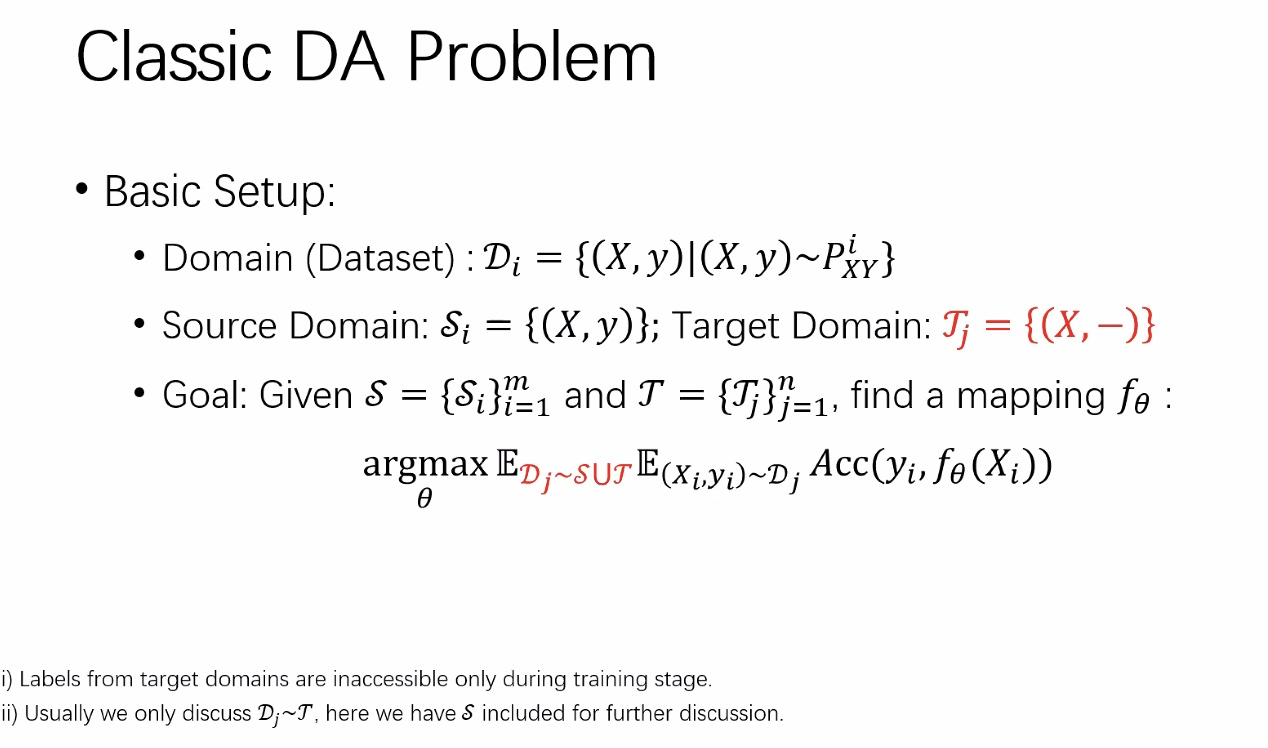
\includegraphics[scale = 0.25]{ClassicDA_Setup.jpg}

Pseudo labeling is important since labeled data becomes inaccessible in later stages. Three types of pseudo label methods include hidden structure based, data augmentation based, and knowledge distillation based. \\

\section{Diverse Reinforcement Learning}

\textit{Led by Pankayaraj Pathmanathan.} \\

\begin{definition}[Diverse RL]
    Diverse RL aims to induce diversity in policies as well as online adapation of the diverse policies. 
\end{definition}

\underline{Problem Formulation: Inducing Diversity}: We want to generate multiple policies so that each policy will be different from each other. Related/previous work includes information based and successor feature based methods.\\

Pan then presents his own ideal method for Diverse RL (details left out, to be presented in future papers). Flaws of previous objective functions include that
\begin{enumerate}
    \item It makes the support for a certain policy weaker.
    \item It adds a level of stochasticity to the overall reward.
\end{enumerate}

He introduces an alternative stable objective function that can be intrepreted as a cross entropy between two distributions with a constant difference. The new objective will be without an indicator function term. With this objective, the stability factor is a bigger factor when it comes to training (even compared to ``ideal'' objectives).
\end{document}